\documentclass[a4paper]{article}

\usepackage[francais]{babel}
\usepackage[T1]{fontenc}
\usepackage[applemac]{inputenc}

\usepackage{geometry}
\usepackage{graphicx}
\usepackage[colorlinks=true]{hyperref}
\hypersetup{urlcolor=blue,linkcolor=black,colorlinks=true}
\usepackage{listings}
\usepackage{amssymb}
\usepackage{setspace}
\usepackage{lscape}
\usepackage[final]{pdfpages}


\pagestyle{headings}
\thispagestyle{empty}
\geometry{a4paper,twoside,left=2.5cm,right=2.5cm,marginparwidth=1.2cm,marginparsep=3mm,top=2.5cm,bottom=2.5cm}

\begin{document}
\large
\setlength{\parskip}{10mm plus2mm minus2mm}
\setlength{\evensidemargin}{-2cm}
\setlength{\textwidth}{530pt}
\setlength{\parindent}{0cm}

21 janvier 2012 \hfill M1 Informatique


{\centering \Large \bfseries Analyse et conception d'algorithmes �conomes en �nergie dans les r�seaux de capteurs \par}

{
Nom du groupe : WSN

�tudiants :
\begin{description}
\item Chlo� DESDOUITS \hfill chloe.desdouits@etud.univ-montp2.fr
\item Sofiane Zahir KALI \hfill zahir.kali@etud.univ-montp2.fr
\item Rabah LAOUADI \hfill rabah.laouadi@etud.univ-montp2.fr
\item Samuel ROUQUIE \hfill samuel.rouquie@etud.univ-montp2.fr
\item
\end{description}

Encadrante : Anne-Elisabeth Baert
\par}
\renewcommand\labelitemi{\textbullet}
{\bfseries Les t�ches r�alis�es � ce jour sont les suivantes :}\\
\begin{itemize}\addtolength{\itemsep}{0.3cm}
	\item Lecture de quelques articles : \cite{Chang2000} \cite{Shah2002} (Chlo� Desdouits), \cite{Cartigny2003LMEB} \cite{Cartigny2005} (Sofiane Zahir Kali), \cite{Ingelrest2005} (Rabah Laouadi), (Samuel Rouquie).
	\item R�sum�s des articles.
	\item Synth�se des connaissances acquises (Samuel Rouquie).
	\item Programmation d'algorithmes sous WSNET :  $FA$ \cite{Chang2000} (Chlo� Desdouits), $LBIP$, $MPR$ et $NES$ (Rabah Laouadi), (Zahir Kali).
\end{itemize}


\begin{landscape}

\begin{figure}
\centering
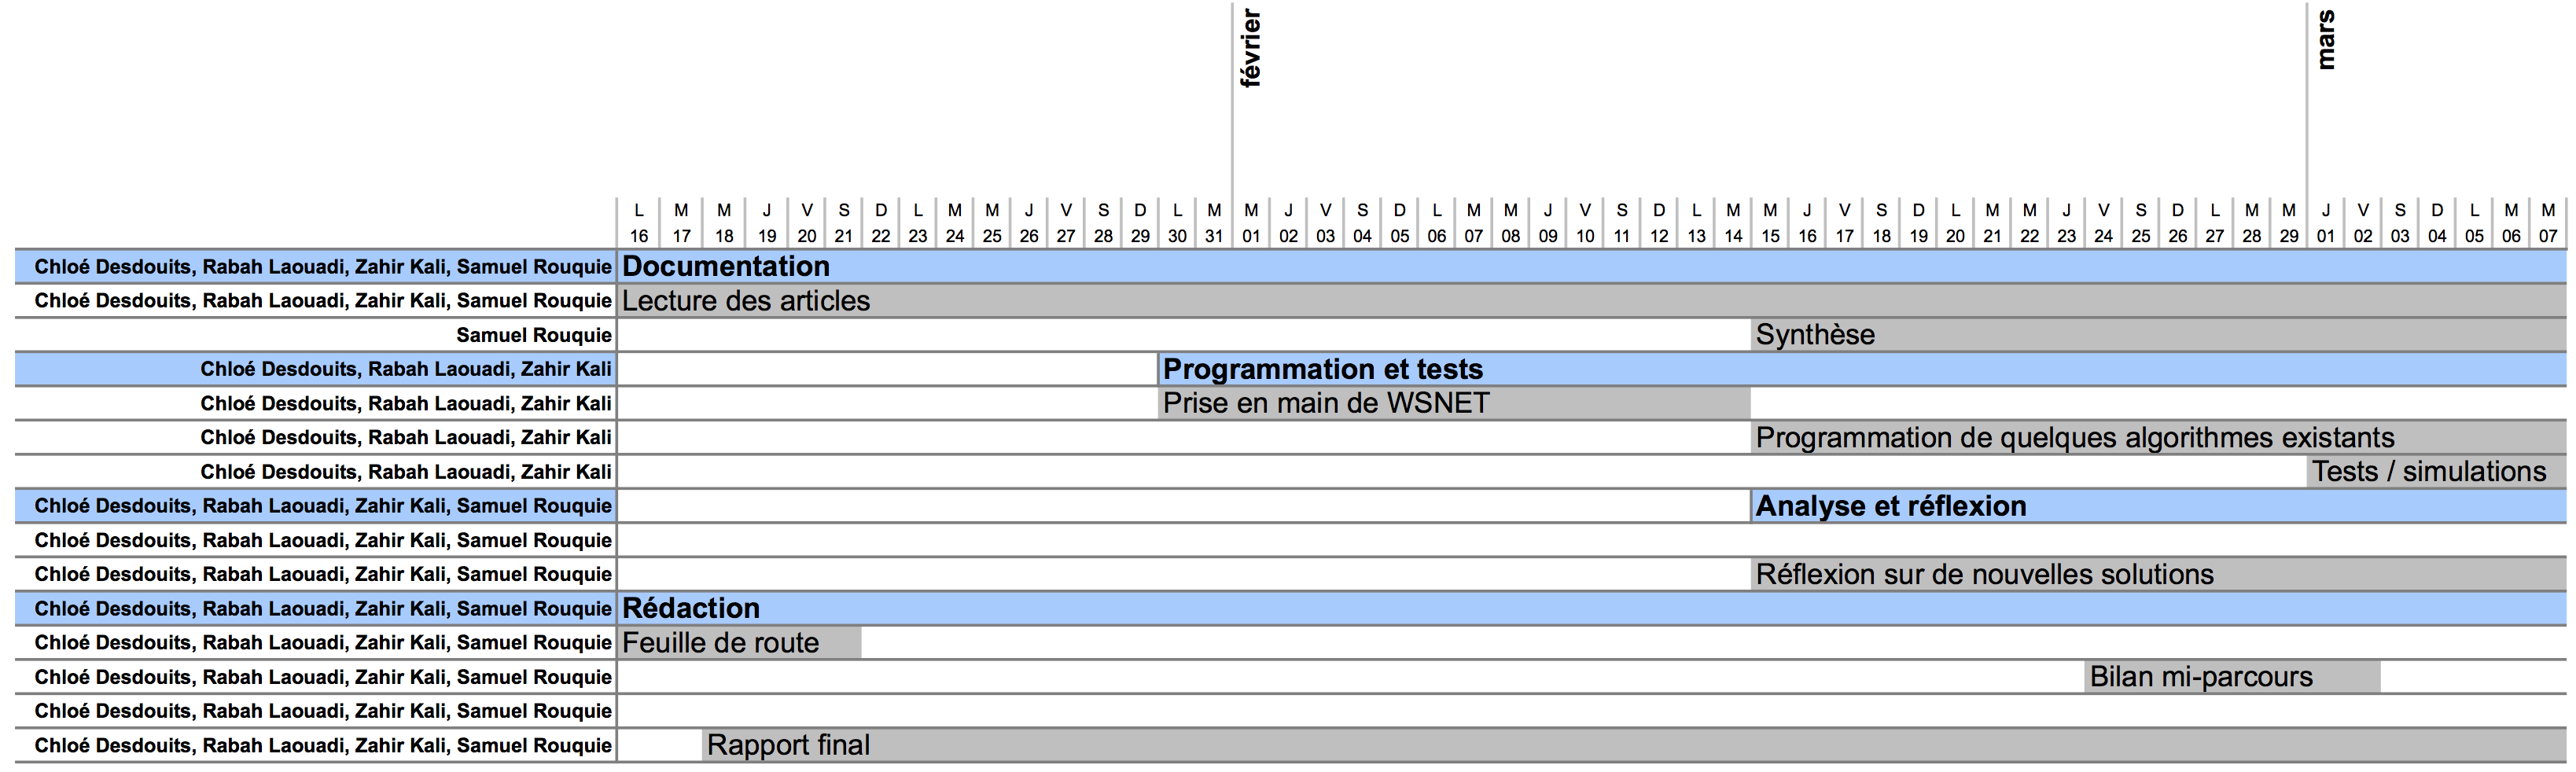
\includegraphics[scale=0.98]{diagramme}
\end{figure}

\begin{figure}
\centering
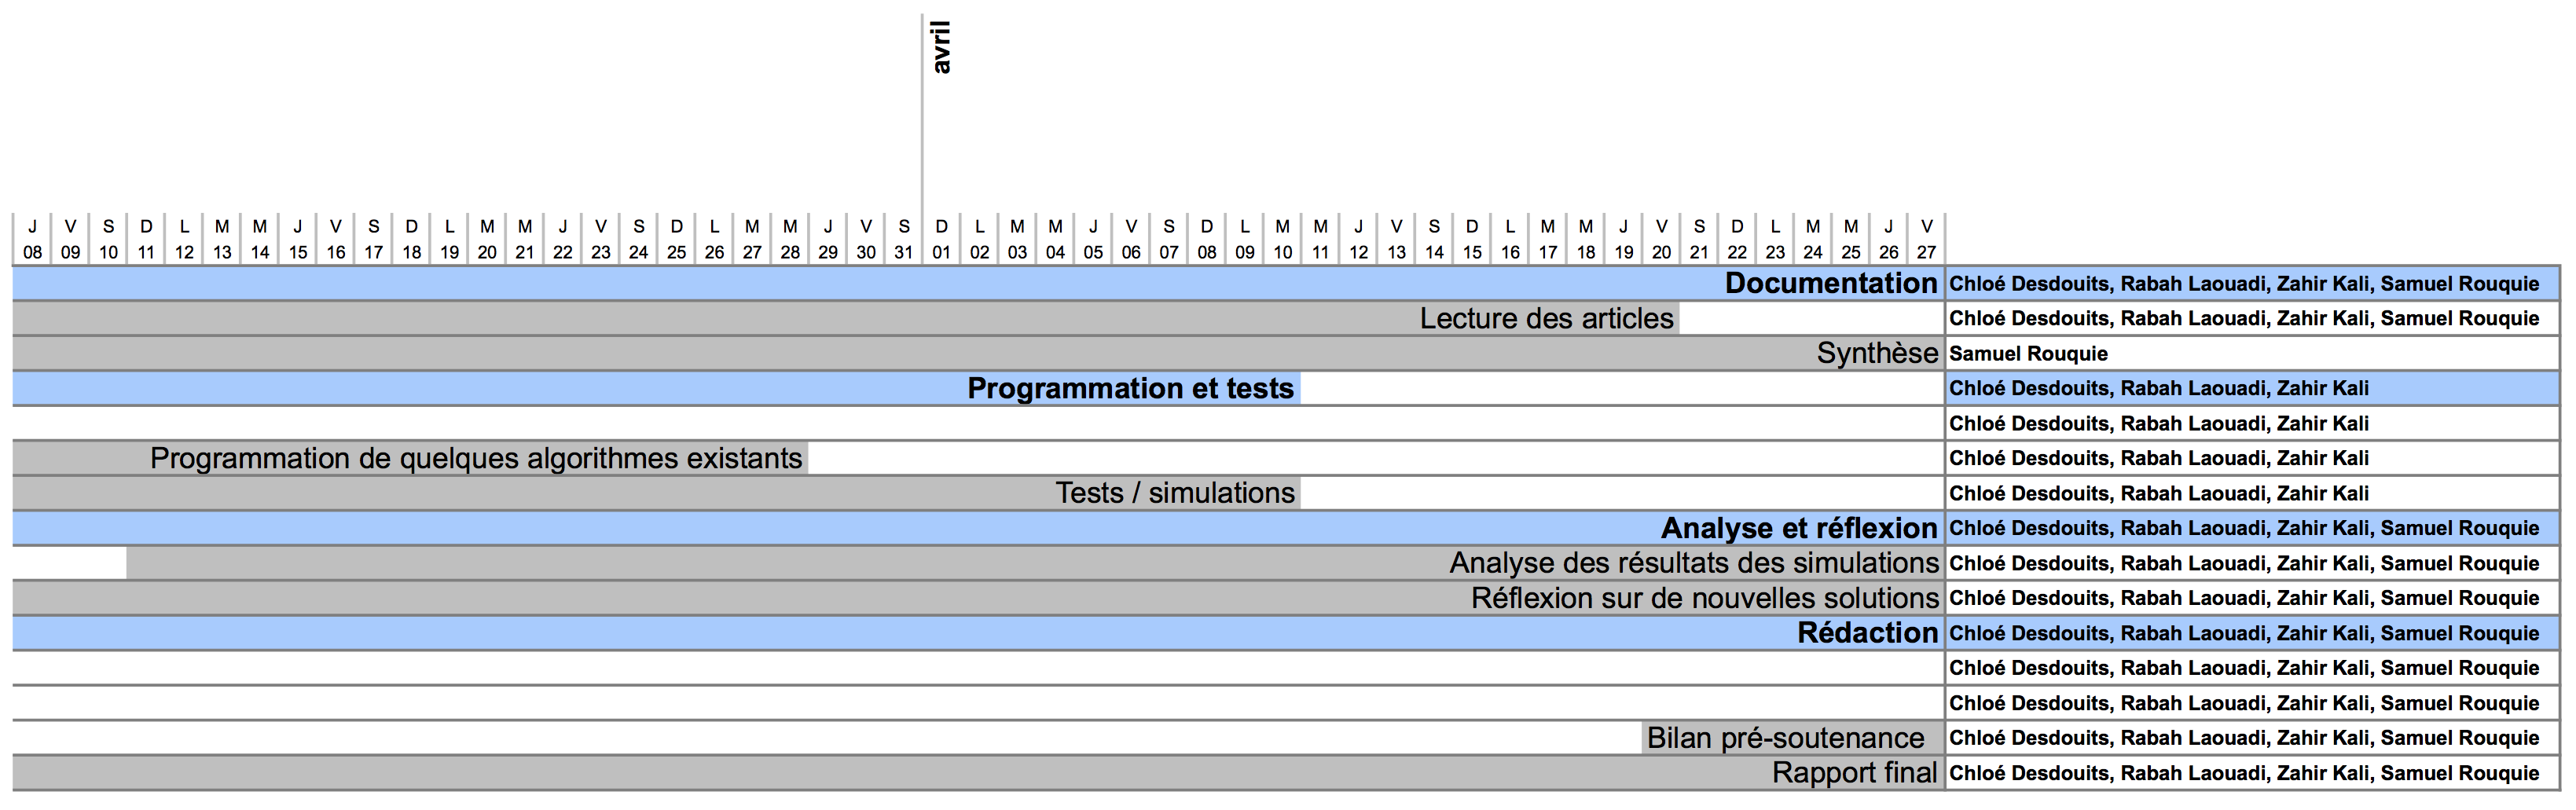
\includegraphics[scale=0.98]{diagramme2}
\end{figure}

\end{landscape}


\bibliographystyle{plain}
\bibliography{../Bib}

\end{document}
